
\chapter{CARBON MONOXIDE-INDUCED ISLAND FORMATION ON PT/PD(557) SURFACE ALLOYS: A MOLECULAR DYNAMICS STUDY}
\label{chap:island}


%\begin{abstract}
%  Stepped surfaces of bimetallic \ce{Pd}/\ce{Pt} alloys were exposed
%  to a range of coverages of adsorbed carbon monoxide (\ce{CO}) using
%  molecular dynamics (MD) simulations. Metal-\ce{CO} interactions for
%  both metals were parameterized from experimental data and Density
%  Functional Theory (DFT) calculations, providing classical potentials
%  that capture the atop binding preference on \ce{Pt} and the
%  hollow/bridge preference on \ce{Pd}.  The MD simulations indicate
%  significant restructuring in the surface alloy, with \ce{Pt}-rich
%  islands forming on the \ce{Pd} substrate within 60~ns.  The
%  time-dependence of the surface domain sizes and the dynamics of
%  nearest-neighbor metal populations suggest that multi-layer \ce{Pt}
%  islands form more rapidly in the presence of adsorbed \ce{CO}.  We
%  find that the different binding preference of \ce{CO} adsorbed to
%  the two metals can help explain the observed stabilization of the
%  \ce{Pd} surface structures as well as the roughening of the \ce{Pt}
%  step edges.  Because the \ce{CO} acts to lower the surface energy of
%  the \ce{Pt}, we conclude that the mechanism for accelerating
%  \ce{Pt}-island formation is kinetic in nature.
%\end{abstract}


In this chapter we explore a bimetallic \ce{Pt/Pd} near surface alloy (NSA)
exposed to \ce{CO} through molecular dynamics simulations. A forcefield
describing the \ce{Pd\bond{-}CO} was parameterized as a part of this work and
a pure \ce{Pd} (557) system was modeled as a control. The differing binding
characteristics of \ce{CO}, site and strength, on the two metals was
hypothesized to lead to significant exposure of the underlying \ce{Pd}
requiring the overlayer of \ce{Pt} to either bury itself or cluster into small
nanostructures on the surface. The stability of the systems and specifically
the \ce{Pt} overlayer was examined as a function of time and \ce{CO} coverage.
Ultimately the binding preference of the \ce{CO} was discovered to play a
primary role in describing the preferred equilibrium states of these systems.


%\section{Introduction}

%Materials based on metallic \ce{Pt} and \ce{Pd} are important
%catalysts for the oxygen reduction
%(ORR)\citep{Lim:2009fk, Liu:2012bs, Limpattayanate:2014ij} and oxygen
%evolution reactions (OER).\citep{Stamenkovic:2007kk, Reier:2012uq} These
%reactions are important in proton-exchange membrane (PEM) fuel
%cells,\citep{Bliznakov:2012kx, Shao:2013rm} as well as in the charging
%and discharging of \ce{Li}-air batteries.\citep{Lu:2011vn}
%Oxide-supported noble metal nanoparticles also play an important role in
%the water-gas shift reaction.\citep{Bunluesin:1998ys, Kugai:2011rt}
%
%However, the expense of \ce{Pt} metal coupled to the slow kinetics of
%the ORR on pure \ce{Pt} or \ce{Pt}/\ce{C} systems remain barriers to
%large-scale implementation of fuel cells. Strategies involving
%bimetallic particles, surface alloys, and core-shell nanostructures
%are currently under investigation in hopes of eliminating these
%barriers.\citep{Gao:2009oj, Gao:2009wo, Kim:2013mi} The coupling of two
%(or more) components in these structures allows for a large accesible
%design space for various catalytic properties, whether that be
%catalytic activity,\citep{Kim:2013mi, Sneed:2014fj, Gu:2015cr} thermal
%stability,\citep{Cao:2010gf, Yang:0pd, Huang:2012ul} or resistance to
%deactivation.\citep{Yu:2013fr, Zhang:2015yq} Specifically,
%\ce{Pt\bond{-}Pd} nanoparticles have been shown to have increased
%activity for the ORR reaction,\citep{Lim:2009fk, Liu:2012bs, Shao:2013rm}
%while \ce{Pt\bond{-}Au} nanoparticles were reported as being more
%stable over repeated potential cycling.\citep{Zhang:2007uq}
%
%Bimetallic \ce{Pt}/\ce{Pd} mixtures also find widespread use in diesel
%oxidation catalysts (DOC) which complete the oxidation of carbon
%monoxide and partially-combusted hydrocarbons, and reduce the nitrogen
%oxides in combustion gases.\citep{Morlang:2005uq, Russell:2011fk}
%\ce{Pd} is a particularly useful metal for diesel catalysts because it
%has a lower intrinsic \ce{SO2} oxidation activity than
%\ce{Pt}.\citep{Russell:2011fk} The \ce{Pt}/\ce{Pd} bimetallic catalyst
%also significantly inhibits sintering of the particles at higher
%temperatures, relative to pure \ce{Pt} catalysts.\citep{Morlang:2005uq}
%
%Catalytic activity is dependent on the exposed structure of \ce{Pt} in
%many of these applications. Reconstruction of the exposed \ce{Pt} can
%therefore change the effectiveness of a given \ce{Pt}-\ce{M} species.
%Of particular interest in diesel oxidation catalysis is carbon
%monoxide (\ce{CO}) and its strong binding affinity for \ce{Pt} and
%\ce{Pd}. Tao \textit{et al.} have shown that the presence of \ce{CO}
%can induce reversible surface reconstructions on a stepped
%\ce{Pt}(557) surface.\citep{Tao:2010aa} Significant experimental and
%theoretical work has been done to more fully characterize the effect
%adsorbed \ce{CO} has on
%\ce{Pt}.\citep{Batteas:1996rc, Thostrup:2001dn, McCarthy:2012qd, Michalka:2013aa, Carenco:2014aa}
%
%This paper describes an investigation into the effects of carbon
%monoxide adsorption on surface restructuring of pure \ce{Pd}(557) and
%\ce{Pt}/\ce{Pd}(557) surface alloys using molecular dynamics
%simulations. Since the long-time dynamics of the restructuring process
%are of particular interest, classical force fields which balance
%computational efficiency against chemical accuracy were employed.

\section{Methodology}
\subsection{Interaction potentials}

%Modeling large metallic interfaces (10\textsuperscript{3}-
%10\textsuperscript{4} atoms) over relatively long time scales (10-100
%ns) requires the use of empirical potentials. Cohesive and surface
%energies in metals are not reproduced with purely pairwise
%interactions, so a number of empirical potentials have been developed
%for modeling transition metals.  These include the embedded atom
%method (EAM)\citep{Foiles:1986ky}, Finnis-Sinclair,\citep{Finnis:1984hl} and
%Sutton-Chen-based models like QSC.\citep{Goddard:1998qsc} These models describe an
%atom as a positively charged core with a radially-decaying valence
%electron density.  Refinements include angle dependent EAM
%implementations,\citep{Baskes:1987aa} that treat BCC metals more
%accurately.
%
%In EAM, the energy for embedding a metallic atom $i$ at a specific
%location in the system requires the electron density at that location,
%\begin{equation*}
%\rho_i = \sum_{j\neq i} \rho_j(r_{ij}).
%\end{equation*}
%This density at site $i$, $\rho_i$ depends on the contributions to the
%electron density from all other atoms in the system.  Here,
%$\rho_j(r)$ describes the distance dependence of the valence electron
%distribution of atom $j$.  Atom $i$'s contribution to the potential
%energy can then be obtained from an embedding functional, $F_i\left[
%  \rho_i \right]$, that depends on $\rho_i$, as well as from a sum of
%pairwise interactions,
%\begin{equation*}
%  V_i =  F[ \rho_i ]  + \sum_{j \neq i} \phi_{ij}(r_{ij})
%\end{equation*}
%
%The embedding energy functional is parameterized for each metallic
%atom type, and depends only on the local electron density, $\rho_i$.
%Thus, the cohesive energy for atom $i$ depends on collective
%contributions from all of the surrounding metal atoms, and is an
%explicitly non-pairwise additive quantity.
As in Chapter \ref{chap:PtAu}, the Embedded-Atom-Method (EAM) was used to model
the metal-metal interactions while the Karplus and Straub model of carbon
monoxide was used to describe the \ce{CO} self interactions. Due to its development, the EAM
method is effective at modeling alloys as the density portion is unchanged
and only the short-ranged repulsions, $\phi$, need to be modified. EAM treats
short-range repulsions as a pairwise contribution that models the repulsive
overlap of the positively-charged cores. For alloys, mixing rules as outlined
by Johnson \citep{Johnson:1989yr} were used to compute the heterogeneous pair
potential,

\begin{equation*} 
\phi_{ab}(r) = \frac{1}{2}
\bigg\{ \bigg(
\frac{\rho_b(r)}{\rho_a(r)}
\bigg) \phi_{aa}(r)
+ \bigg(
\frac{\rho_a(r)}{\rho_b(r)}
\bigg)\phi_{bb}(r) 
\bigg\}
\end{equation*} 

In this work, we have employed the embedded atom method (EAM) to describe the
\ce{Pt} and \ce{Pd} electron densities, embedding functionals, and pair
potentials,\citep{Foiles:1986ky} utilizing the Johnson mixing rules for the
\ce{Pt\bond{-}Pd} cross-interactions.\citep{Johnson:1989yr}

The \ce{Pt\bond{-}CO} interactions have been modified from 
fits in Chapter \ref{chap:PtAu} to account for recently-published DFT
data.\citep{Deshlahra:2012aa} This modification yields a slightly weaker
\ce{Pt\bond{-}CO} binding energy, but maintains the atop site
preference.  The potential energy for the interaction of one \ce{CO}
molecule with one metal atom,
\begin{equation*}
V_\mathrm{M\mhyphen CO} = 4 \epsilon \left(
  \left(\frac{\sigma}{r_\mathrm{M\mhyphen C}}\right)^{12} -
  \left(\frac{\sigma}{r_\mathrm{M\mhyphen C}}\right)^6 \right) +
D e^{-2 \gamma (r_\mathrm{M\mhyphen O} - r_e)}
\label{eq:pot}
\end{equation*}
is modeled using a Lennard-Jones interaction between the metal atom
(M) and the carbon along with a repulsive Morse potential between the
metal atom and the oxygen.

Both the \ce{Pd\bond{-}CO} and \ce{Pt\bond{-}CO} interaction
potentials were parameterized as part of this work. The basic model,
using a full Morse potential between the metal and oxygen site and a
Lennard-Jones interaction between the metal and the carbon site, was
introduced by Korzeniewski \textit{et al.}\citep{Korzeniewski:1986kl} One key
difference from the potential in Refs.\citep{Korzeniewski:1986kl} and our
earlier fits in Refs.\citep{Michalka:2013aa} is that the
\ce{M\bond{-}O} bond is modeled here using a purely repulsive Morse
potential. The parameters were fit to reflect binding energies and
binding site preferences on the \ce{M}(111) surfaces.  The functional
forms and the broad repulsive \ce{M\bond{-}O} contribution are
flexible enough to reproduce the atop preference for \ce{Pt\bond{-}CO}
as well as the bridge/hollow preference for \ce{Pd\bond{-}CO}.
Parameters for the potentials are given in
Table~\ref{tab:CO_parameters} and the calculated binding energies at
various binding sites are shown in Table~\ref{tab:CO_energies}.

\begin{table} 
\caption{PARAMETERS FOR THE PT-CO AND PD-CO CROSS-INTERACTIONS}
%\caption{Parameters for the M-\ce{CO} cross-interactions. Metal-Carbon
%  interactions are modeled with Lennard-Jones potentials, while the
%  metal-Oxygen interactions are fit using repulsive Morse potentials.
%  Distances are given in \AA~and energies in
%  kcal/mol.\label{tab:CO_parameters}}
\centering
\begin{threeparttable}  
\centering
\begin{tabular}{ c  cc  c  ccc }
\hline
\hline
 &  $\sigma$\tnote{a} & $\epsilon$\tnote{b} & & $r$\tnote{a} & $D$\tnote{b} & $\gamma$ (\AA$^{-1}$) \\
\midrule
\textbf{\ce{Pt\bond{-}C}} & 1.41 & 45  & \textbf{\ce{Pt\bond{-}O}} & 4.4  & 0.05 & 1.8 \\
\textbf{\ce{Pd\bond{-}C}} & 1.6 &  40  & \textbf{\ce{Pd\bond{-}O}} & 4.95 & 0.05 & 1.45\\
\hline
\hline
\end{tabular}
\begin{tablenotes}
  \item Metal-C interactions are modeled with Lennard-Jones potentials, while the metal-O interactions were fit to Morse potentials.
  \item[a] Distances are given in \AA
  \item[b] Energies are given in kcal/mol
\end{tablenotes}
\end{threeparttable}
\label{tab:CO_parameters}
\end{table}

%Table of energies
\begin{table}
  \caption{ADSORPTION ENERGIES FOR A CO MOLECULE AT THE THREE PRIMARY BINDING SITES ON M(111)}
%  \caption{Single-site adsorption energies for a \ce{CO} molecule at
%    the three binding sites on \ce{M}(111) using the potentials
%    described in Table \ref{tab:CO_parameters}.  These values are
%    compared with 
%    electronic structure and experimental desorption
%    data when available. Note that the electronic structure values are
%    for surface 
%    coverages of $\ge$ 0.25 ML, and
%    experimental values are (in most cases) extrapolated to zero
%    coverage from desorption energies at higher coverages.  All values
%    are in eV.}
\centering
\begin{threeparttable}
\begin{tabular}{ c  ccc  c }
  \hline
  \hline
  & Site & This Model\tnote{a} & DFT\tnote{a} & Experimental\tnote{a} \\
  \hline
  \textbf{\ce{Pt\bond{-}CO}} & atop   & -1.47 & -1.48\citep{Deshlahra:2012aa} & -1.39\citep{Kelemen:1979ad}, -1.43\citep{Ertl:1977cg}, -1.90\citep{Yeo:1997th} \\
                 & bridge & -1.13 & -1.47\citep{Deshlahra:2012aa} &  \\
                 & hollow & -1.02 & -1.45\citep{Deshlahra:2012aa} &  \\
\hline
  \textbf{\ce{Pd\bond{-}CO}} & atop   & -1.54 & -1.44\citep{Honkala:2001sf} &  \\
                 & bridge & -1.65 & -1.83\citep{Honkala:2001sf} &  \\
                 & hollow & -1.60 & -1.99\citep{Honkala:2001sf} & -1.30\citep{Szanyi:1992aa}, -1.47\citep{Ertl:1970aa}, -1.54\citep{Guo:1989aa} \\
  \hline
  \hline
\end{tabular}
\begin{tablenotes}
  \item The energies are obtained using the potentials described in Table \ref{tab:CO_parameters}. These values are compared with electronic structure and experimental desorption data when available Note that the electronic structure values are for surface coverages of $\ge$ 0.25 ML, and experimental values are (in most cases) extrapolated to zero coverage from desorption energies at higher coverages.
  \item[a] All values are in eV
\end{tablenotes}
\end{threeparttable}
\label{tab:CO_energies}
\end{table}

This \ce{Pd\bond{-}CO} model does not have a strong preference for
either the bridge or hollow binding sites, so it may overestimate the
bridge-site binding at low coverages, but at higher coverages, the
experimental situation is somewhat less clear.\citep{Wong:1991ta}
Studies using low-energy electron diffraction (LEED) and
\ce{C\bond{-}O} stretching frequencies of \ce{CO} bound to
\ce{Pd}(111) suggest that the 3-fold hollow sites are preferred at low
coverages,\citep{Bradshaw:1978uf, Conrad:1978fx, Ohtani:1987zh} where it
forms a $(\sqrt{3} \times \sqrt{3}) R~30^{\circ}$ pattern.  These
observations are supported by temperature desorption
spectroscopy,\citep{Guo:1989aa} and infrared absorption
spectroscopy~\citep{Szanyi:1992aa} where binding energies have been
reported to lie between -1.3 and -1.54 eV.

At higher \ce{CO} coverages (e.g. $> 0.5$ ML), the preferred binding
of \ce{CO} on \ce{Pd}(111) appears to be a $c(4\times2)$ ordered
structure with the \ce{CO} bound to the bridge
sites.\citep{Bradshaw:1978uf} 

Theoretical work by Honkala \textit{et al.}\citep{Honkala:2001sf} using
DFT with the generalized gradient approximation (GGA) to describe
electron exchange correlation and pseudopotentials for the \ce{Pd}
atoms also reported the fcc site as the most favorable binding
position with a binding energy of -2.00 eV compared to the bridge site
binding energy of -1.83 eV at 0.33 monolayer.

High resolution x-ray photoelectron spectroscopy (XPS) results from
Surnev \textit{et al.}\citep{Surnev:2000uk} confirm that the preferred
low coverage ($< $ 0.1 ML) binding site is the fcc hollow, but also
suggest a competition between hollow and bridge binding for coverages
between 0.1 and 0.32 ML, suggesting similar binding energies for these
two sites. Additional DFT calculations from Loffreda \textit{et
al.}\citep{Loffreda:1999vl} suggest that as the coverage increases, the
binding energy difference shrinks, as at 0.5 ML the hollow to bridge
energy difference is 0.06 eV (-1.85 hollow, -1.79 bridge).

Although the weak preference for hollow vs. bridge sites at low
coverage is not captured by the \ce{Pd\bond{-}CO} fit, at low
temperatures on \ce{Pd}(111), a 0.5 ML coverage of \ce{CO} interacting
with the potential in Table \ref{tab:CO_parameters} does produce
domains with the $c(4\times2)$ ordered structure (see 
appendix \ref{app:SI}).

Experimental work on CO on Pt(111) using LEED has suggested that the
atop binding is 70 meV stronger than the bridge
site~\citep{Schweizer:1989fk} and forms a
$(\sqrt{3} \times \sqrt{3}) R~30^{\circ}$ structure on solely atop
sites at low surface coverages.\citep{Kelemen:1979ad} Because our Pt-CO
model uses relatively long-range repulsive Morse interactions to
preserve the CO orientation on the surface, it overestimates the atop
binding preference relative to the DFT calculations.  However, the
model is able to reproduce small domains of the
$(\sqrt{3} \times \sqrt{3}) R~30^{\circ}$ structures (see 
appendix \ref{app:SI}).

\subsection{(557) Interfaces and surface alloys}
The \ce{Pd}(557) model is contained in an orthorhombic periodic box
with dimensions of $55.09 \times 49.48 \times 120$~\AA~ while the
surface alloys (\ce{Pt}(557) surface layers, with \ce{Pd} bulk) have
dimensions of $54.875 \times 49.235 \times 120$~\AA.  The \ce{Pd}
system consists of 9 layers of \ce{Pd} while our surface alloys
consist of 7 layers of \ce{Pd} sandwiched between 2 single layers of
\ce{Pt}.  Both the pure \ce{Pd} slab and the surface alloy systems are
$\sim$22~\AA~ thick. The lattice constants for \ce{Pd} and \ce{Pt},
3.89 and 3.92~\AA, respectively, result in minimal strain energy in
the alloy, and the relaxed geometries of the two interfaces are
therefore quite similar.

The systems are cut from a FCC crystal along the (557) plane, and are
rotated so that they are periodic in the $x$ and $y$ directions,
exposing (557) facets on both the positive and negative sides of the
$z$-axis of the box.

Simulations of the metal without any adsorbate present were performed
at temperatures ranging from 300 to 900~K to establish the stability
of the (557) surface without a \ce{CO} overlayer.  The bare systems
were run in the canonical (NVT) ensemble at 850~K for 200~ps and the
microcanonical (NVE) ensemble for 1~ns, and displayed minimal changes
in the (557) structure during this period.  This temperature is well
below previously simulated melting temperatures for \ce{Pt}/\ce{Pd}
alloyed nanoparticles in both free and graphite-supported
configurations.\citep{Sankaranarayanan:2005bh, Sankaranarayanan:2005qf, Fernandez:2013yg}

Ten systems were constructed, corresponding to five \ce{CO}-coverage
levels for each metallic system.  The number of \ce{CO} molecules (0,
48, 240, 320, and 480) yield surface coverages of approximately 0,
0.05, 0.25, 0.33, and 0.5 monolayers (ML) assuming that every \ce{CO}
adsorbs on the surface.

Simulation boxes of the same sizes as the metallic systems were
constructed with appropriate densities of \ce{CO} and equilibrated to
850~K. The gas-phase \ce{CO} and surface simulation boxes were then
combined, using a 5~\AA\ cutoff between metallic atoms and \ce{CO} to
prevent overlap. The remaining \ce{CO} population was further reduced
to match the required number for the correct surface coverage.
Velocities were resampled from a Boltzmann distribution, and any net
linear momentum was subtracted from the entire system.  The combined
systems were run for 1~ns in the NVT ensemble, before being run in the
NVE ensemble for data collection.  The \ce{CO} molecules were
initially introduced in the gas phase and were allowed to freely
adsorb and migrate on the surface.  In most cases, the \ce{CO}
adsorbed on the metal surfaces within the first 100~ps of the initial
1~ns equilibration time.

All of the \ce{Pd} systems were run in the microcanonical ensemble for
a minimum of 40~ns to collect statistics. The \ce{Pt}/\ce{Pd} surface
alloy systems, which were observed to undergo significant
restructuring, were each run for a total simulation time of 113~ns.
All simulations were carried out with the open source molecular
dynamics package, OpenMD.\citep{openmd, Meineke:2005pt}
 
\subsection{Analysis of surface features and adatom diffusion}
To analyze surface domain sizes, the exposed surfaces (both top and
bottom of the slabs) were first projected onto 2-dimensional square
grids with 1~\AA\ grid spacing. The grid points were assigned
``\ce{Pt}'' or ``\ce{Pd}'' values based on the identity of the closest
surface atom.  The grids were then separated into contiguous domains
using nearest-neighbor similarity (i.e., the four nearest grid
points). The resulting domain areas were averaged over 18~ns windows.
A representative grid decomposition is shown in fig. \ref{fig:grid}.

\begin{figure}[p!]
  \includegraphics[width=\linewidth]{../figures/chap3/coloredGrid.pdf}
  \caption{Analysis of the surface alloy to find surface domain sizes
    was carried out by mapping the surface composition (left) onto
    1~\AA\ spaced grid points (center).  Contiguous domains were
    identified and have been shown in distinct colors (right), and the
    distribution of domain areas was collected over 18~ns time
    windows.}
\label{fig:grid}
\end{figure}

To estimate the surface diffusion constants, we define a mobile atom
as one which moves at least 2~\AA\ in any 10~ps window during a 10~ns
segment of simulation time.  The fraction of exposed surface atoms
that met this criteria defines the mobility fraction,
$f_\mathrm{mobile}$.  For the mobile atoms, diffusion constants were
calculated in 10~ns windows to follow changes in adatom transport
after the initial exposure to \ce{CO}.

\section{Results}
\subsection{Structural changes}
On \ce{Pt}(557), we previously observed \ce{CO}-induced restructuring
into relatively clean double-layer structures.\citep{Michalka:2013aa} For
the pure \ce{Pd}(557) studied here, the (557) facet retains the (111)
plateaus and (100) steps with only minimal adatom movement, and with
almost no surface reconstruction.  Higher \ce{CO} coverages appear to
have minimal effect (and may even stabilize the steps) when compared
with the bare \ce{Pd}(557) systems.

The \ce{Pt}-coated \ce{Pd} surface alloy exhibits a \ce{CO}-induced
speedup of \ce{Pt}-adatom diffusion, as well as a large-scale
restructuring of the well-ordered surface into \ce{Pt}-rich islands.
This surface will therefore be the focus of most of our analysis.

\begin{figure}[p!]
  \includegraphics[width=\linewidth]{../figures/chap3/pinkGray.pdf}
  \caption{Snapshots of some of the simulated systems highlighting the
    (557) step edges (top) along with a diagonal view (bottom).
    System (a) is the pure \ce{Pd} (557) $\sim$40~ns after being dosed
    with 0.5~ML of \ce{CO}.  System (b) is the bare surface alloy
    after $\sim$110~ns at 850~K, while (c) is the surface alloy
    $\sim$110~ns after exposure to 0.5~ML of \ce{CO}.  \ce{Pt} atoms
    are shown in gray, \ce{Pd} in pink, while the adsorbed \ce{CO}
    molecules are shown in silver / red.}
\label{fig:systems}
\end{figure}

Figure \ref{fig:systems} shows representative configurations of the
various systems after significant exposure to the \ce{CO}. We see that
the \ce{Pd} system highlighted in panel (a) has undergone no surface
restructuring. The other panels highlight the effect of varying
\ce{CO} concentrations on the surface alloys, which do exhibit
structural reorganization.

\subsection{Transport of surface metal atoms}

Figure \ref{fig:systems} suggests that there is limited to no mobility
on the pure \ce{Pd} systems. Analysis of the surface atom mobility
showed that fewer than 6\% of the surface \ce{Pd} atoms made $> 2$~\AA\
hops in any 10~ps window during the entire 40~ns run. As most of these
atoms immediately hopped back to their starting points, surface
diffusion constants on \ce{Pd}(557) are as close to zero as can be
safely estimated.

However, there is significant movement of surface \ce{Pt} in the alloy
systems, and the mobility of the surface \ce{Pt} layer increases with
increasing \ce{CO} coverage. The initial 50~ns of exposure is
far from equilibrium, and adatom diffusion constants stabilize after
this 50~ns period.  The diffusion constants shown in Table
\ref{tab:diffusion} are calculated from the last (equilibrated) 60 ns
of each simulation. The fraction of mobile surface atoms grows
linearly with increasing \ce{CO} coverage from 27\% of the bare metal
surface with no \ce{CO} overlayer to 33\% of the surface metal atoms
under 0.5 ML of \ce{CO}.

\begin{table} 
\caption{FRACTION OF MOBILE PT SURFACE ATOMS AND THEIR SURFACE DIFFUSION}
\centering
\begin{threeparttable} 
\centering
\begin{tabular}{ccc} 
\hline
\hline
    \ce{CO} Coverage & $f_\textrm{mobile}$  & $D$ (\AA\textsuperscript{2}/ns) \\
\hline
    0.00 & 0.27(1) & 1.1(3) \\
    0.05 & 0.28(2) & 1.2(3) \\
    0.25 & 0.30(2) & 1.3(3) \\
    0.33 & 0.37(2) & 1.7(3) \\
    0.50 & 0.33(3) & 1.0(2) \\
\hline
\hline
\end{tabular}
\begin{tablenotes}
  \item The fraction of mobile \ce{Pt} surface atoms
    ($f_\textrm{mobile}$) and surface diffusion constants ($D$) for the
    surface alloys as a function of the \ce{CO}
    coverage
  \item Uncertainties in the last digit are shown in parentheses
\end{tablenotes}
\end{threeparttable}
\label{tab:diffusion}
\end{table}

\subsection{Pt island formation on the Pt/Pd alloy}

At the beginning of the simulations, the surface layer of \ce{Pt} made
up one domain of $\sim$2625~\AA\textsuperscript{2}. In all
simulations, this domain broke up relatively quickly and was matched
by a growth in the number and size of \ce{Pd} domains. The presence of
\ce{CO} in the system increased the clustering of the \ce{Pt} domains,
with a concomitant exposure of the underlying \ce{Pd}.

The structural reconstructions that occur for the surface alloy are
influenced by the presence of the \ce{CO} adsorbate. In Figure
\ref{fig:domainAreasPd}, the area of exposed \ce{Pd} increases both
over time, and as a function of \ce{CO} coverage.  The presence of
\ce{CO} increases exposure of the underlying \ce{Pd}, as measured by
the number and sizes of exposed \ce{Pd} domains. Without \ce{CO}
exposure, the bare \ce{Pt}/\ce{Pd} surface does undergo some
restructuring at 850~K, although both the rate and extent is
significantly smaller than in the 0.25 and 0.50 monolayer (ML)
systems.

\begin{figure}[p!]
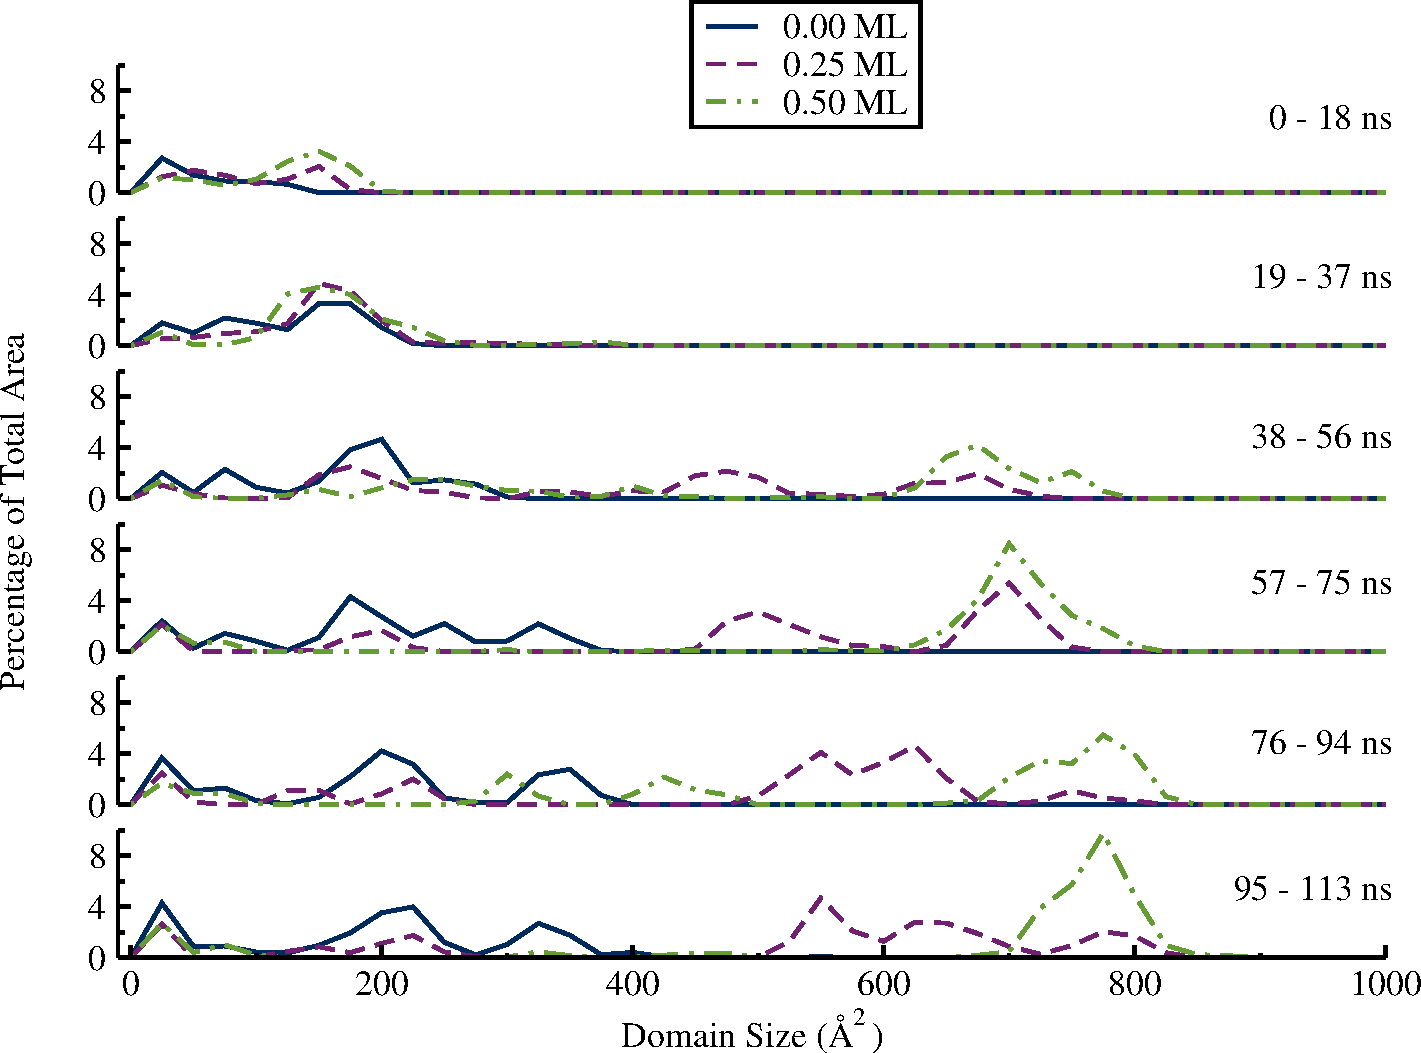
\includegraphics[width=\linewidth]{../figures/chap3/domains_Pd_110ns.pdf}
\caption{Distributions of \ce{Pd} domain sizes at different \ce{CO}
  coverages and at different times after exposure to \ce{CO}.}
\label{fig:domainAreasPd} 
\end{figure}

The appearance of \ce{Pd} from the bulk layers on the surface requires
a simultaneous reduction in the surface area of the outer \ce{Pt}
skin. Two scenarios could explain the reduction of exposed \ce{Pt}:
either the \ce{Pt} atoms are being buried under the \ce{Pd} bulk, or
islands of \ce{Pt} are forming on top of the \ce{Pd} surface.

Both mechanisms would explain the decreased \ce{Pt} surface area (see
Fig.  \ref{fig:domainAreasPt}).  To discern which of these mechanisms
is taking place, the identity of nearest metal atom neighbors can be
tabulated as a function of time of exposure to \ce{CO}. Single-layer
\ce{Pt} skins have atoms with 6 \ce{Pt} nearest neighbors. Islands of
\ce{Pt} require the presence of \ce{Pt} atoms with 7-9 \ce{Pt} nearest
neighbors. In figure \ref{fig:nearestNeighbors}, we see an increase in
\ce{Pt} population with 9 \ce{Pt} nearest neighbors along with the
simultaneous decrease in \ce{Pt} atoms with only 6 \ce{Pt} nearest
neighbors.  This is evidence for the formation of multi-layer \ce{Pt}
features since single layers of \ce{Pt} are restricted to having 6
\ce{Pt} nearest neighbors.

\begin{figure}[p!]
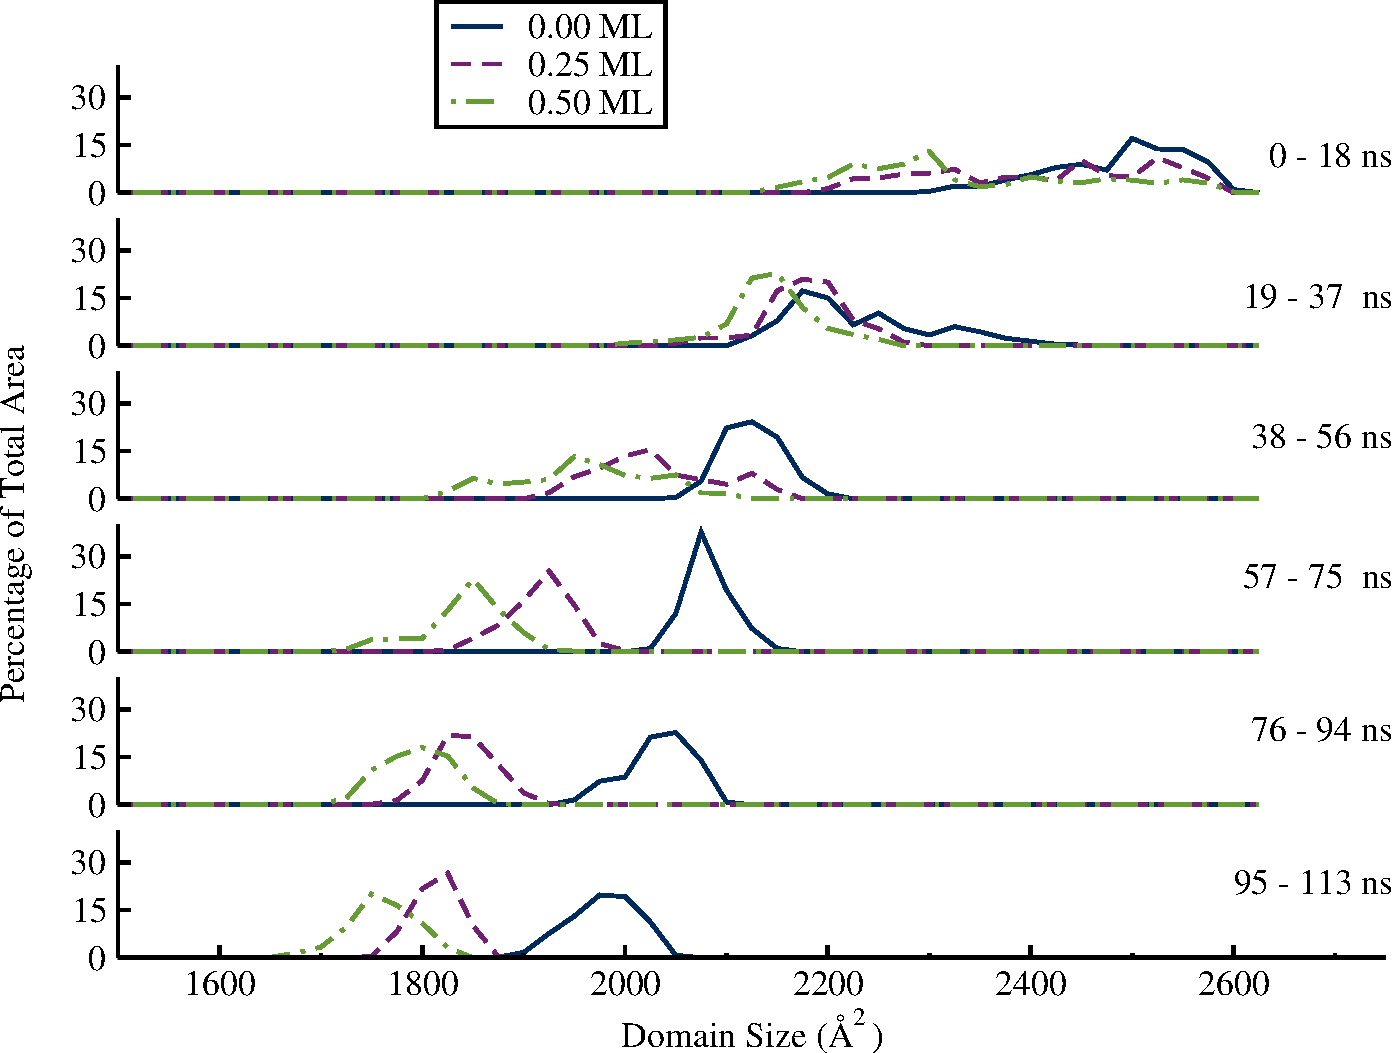
\includegraphics[width=\linewidth]{../figures/chap3/domains_Pt_110ns.pdf}
\caption{Distributions of \ce{Pt} domain sizes at different \ce{CO}
  coverages and at different times after exposure to \ce{CO}.}
\label{fig:domainAreasPt}
\end{figure}

Although it is not shown in Figure \ref{fig:domainAreasPt}, there is
an additional small peak in the \ce{Pt} graphs around 0-100~\AA,
corresponding to 1 to 2 atom clusters of \ce{Pt} embedded in the
\ce{Pd} matrix.  A figure showing the full scale of domain sizes is
supplied in appendix \ref{app:SI}.  The integrated area of
\ce{Pd}
surface coverage for each time window is shown in Table
\ref{tab:integratedArea}.

\begin{figure}[p!]
  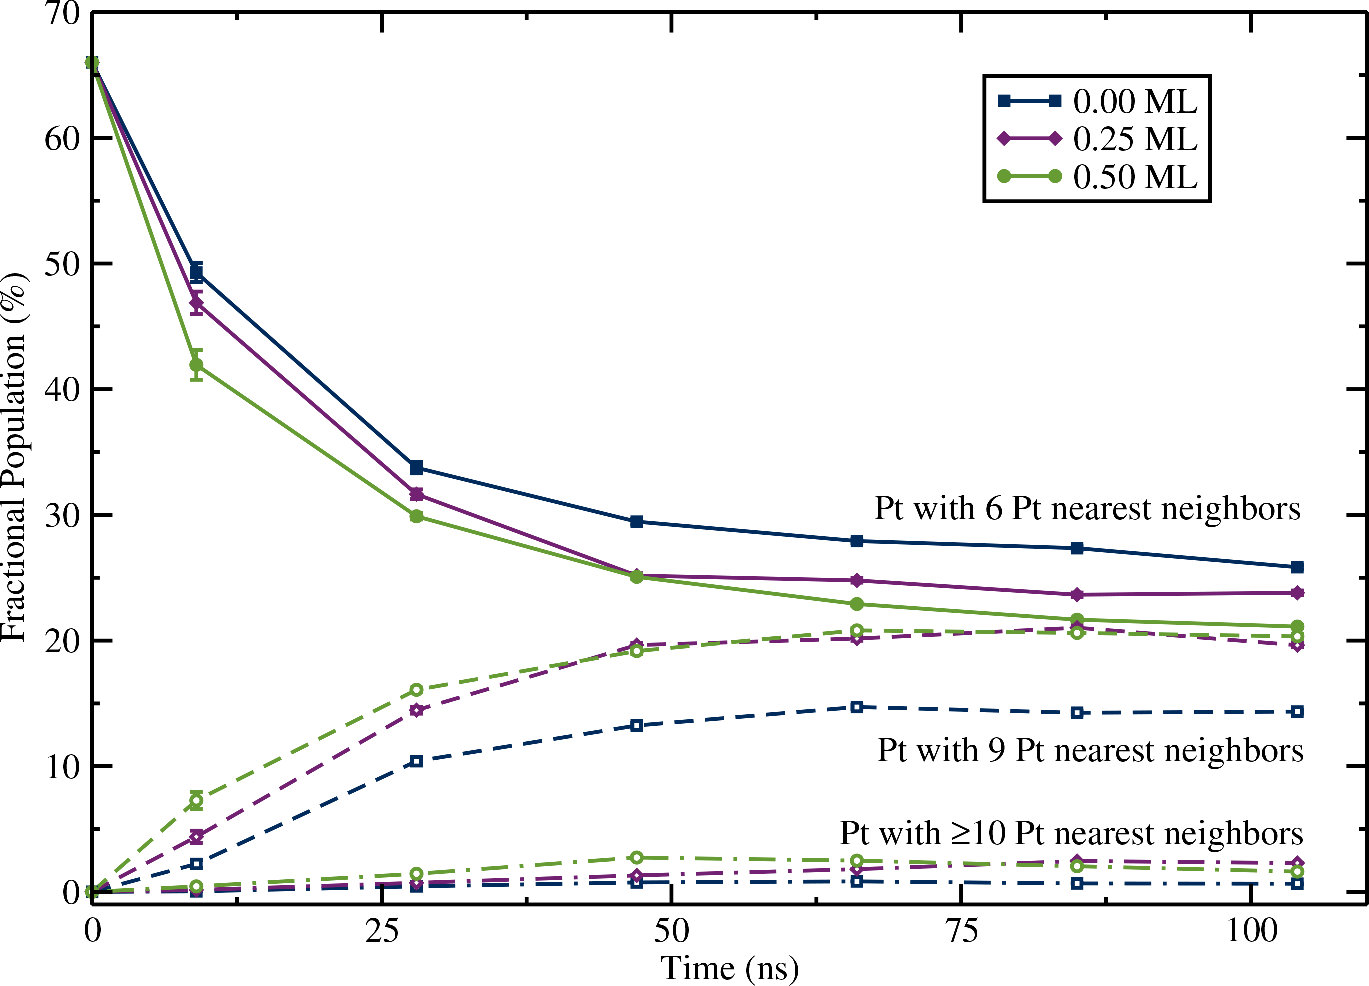
\includegraphics[width=\linewidth]{../figures/chap3/nn.pdf}
  \caption{Population of \ce{Pt} atoms with either 6 (solid), 9
    (dashed), or $\ge$ 10 (dot-dashed) \ce{Pt} nearest neighbors
    averaged over 18 ns blocks of time.  At $t=0$, the majority
    (2/3) of \ce{Pt} is located in the (111) plateaus where
    the number of \ce{Pt} nearest neighbors is 6. The remaining
    \ce{Pt} is located at step edges, with a nearest neighbor \ce{Pt}
    count of 5.} 
\label{fig:nearestNeighbors}
\end{figure}

The presence of \ce{CO} therefore appears to facilitate the clustering
of \ce{Pt} into smaller domains by forming multilayer features which
leads to a reduction of \ce{Pt} surface coverage and concomitant
increased exposure of the underlying \ce{Pd}. We note that
nearest-neighbor population analysis provides information similar to
the information one might obtain from an XAFS experiment, which could
make this phenomenon experimentally observable.

The slower restructuring observed in the bare metal system suggests
that the relative surface energies of the two metals provides the
driving force for the restructuring, while the \ce{CO} significantly
speeds up the effects (and may help to catalyze the process at lower
temperatures).

\begin{table}
%  \caption{\ce{Pd} surface coverage (as a percentage of total surface area)
%    averaged over 18 ns blocks of time.}
  \caption{CHANGE IN PD SURFACE COVERAGE AS A FUNCTION OF TIME AND CO COVERAGE}
  \begin{threeparttable}
  \begin{tabular}{c | c  c  c  c  c  c }
    \hline
    \hline
    \ce{CO} coverage  & 0-18 ns & 19-37 ns & 38-56 ns & 57-75 ns & 76-94
    ns & 95-113 ns \\
    \hline
    0.00 &  6.6 & 16.2 & 20.1 & 21.7 & 23.5 & 25.2  \\
    0.05 &  8.0 & 15.8 & 20.2 & 25.1 & 27.6 & 30.9  \\
    0.25 &  8.5 & 17.3 & 23.7 & 27.8 & 30.5 & 31.0  \\
    0.33 &  8.8 & 17.8 & 21.9 & 26.2 & 30.3 & 35.4  \\
    0.50 & 11.8 & 19.2 & 25.9 & 29.8 & 31.1 & 32.6  \\
    \hline
    \hline
  \end{tabular}
  \begin{tablenotes}
    \item The amount of Pd surface coverage is shown as a percentage of the total surface area. The individual data points are averaged over 18 nanosecond blocks of time.
  \end{tablenotes}
\end{threeparttable}
\label{tab:integratedArea}
\end{table}

Because many of the changes, both in domain size and in \ce{Pt}-atom
neighborship slow after 50~ns, this timescale appears to indicate the
onset of stable surface structures.  The presence of adsorbed \ce{CO}
hastens the onset of this quasi-equilibrium, although there is
insufficient data to predict rates from our simulations. 

\section{Discussion}

\subsection{Structural changes}

In our previous work on \ce{Pt}(557) surfaces,\citep{Michalka:2013aa} the
surface exhibited a \ce{CO}-induced structural transformation from
single steps to double steps, where the (111) plateaus effectively
doubled in size. The step coherence and orientation was preserved
following the transformation.  In the alloy case studied here, the
\ce{Pt} atoms start to cluster, breaking up the steps and causing
significant disorder on the surface.  We note, however, that the
underlying \ce{Pd} maintains the step-like structures of the (557)
interface.  A figure showing how the underlying \ce{Pd}(557) survives
the surface island formation is supplied in appendix \ref{app:SI}.


The EAM potential predicts surface energies for \ce{Pd} (111), (100),
and (110) facets that are roughly 84\% of the surface energies for the
same facets on bare \ce{Pt}.\citep{Foiles:1986ky} Although the absolute EAM
surface energies differ significantly from experimental values, the
\ce{Pd}:\ce{Pt} surface energy ratio is similar to experimental
results.\citep{Tyson:1977xe, De-Boer:1988tg} All-electron full potential
linearized augmented plane-wave (FP-LAPW) calculations have also
yielded a 0.84:1 ratio between the \ce{Pd}:\ce{Pt} (111) surface
energies.\citep{Silva:2006fk} The (557) interface has broad steps of
exposed (111), so we expect the ratio between the \ce{Pd}:\ce{Pt}
(557) surface energies to also fall close to this 0.84:1 ratio.

Because \ce{Pt} has a higher surface energy, the alloy system will
experience a driving force towards arrangements that minimize the
\ce{Pt} surface area.  Although the \ce{Pt} island formation appears
to be accelerated by the presence of adsorbed \ce{CO}, the
relationship between \ce{CO}-adsorption and the surface energies was
not initially clear. In the sections below, we discuss the effects
that the bound-\ce{CO} has on step edge stability and surface
diffusion.

We note that on \ce{Pt}(557), \ce{CO} aids in double layer formation
by lowering the barrier for an adatom on the lower plateau to burrow
into a nearby step edge.\citep{Michalka:2013aa} This burrowing lifts one
of the step edge atom onto the step above.  On the alloy surface, this
same mechanism can explain the thickening of the \ce{Pt} island layers
that is required by the 9-nearest neighbor clustering in
fig.\ref{fig:nearestNeighbors}.

\subsection{Surface adatom formation}
There is limited movement of \ce{Pd} in all of the systems we
examined. Inversions, where \ce{Pd} and \ce{Pt} atoms are swapped
between surface and subsurface layers, were observed only rarely in
the \ce{Pd}/\ce{Pt} shell, and overall the \ce{Pd} is largely
stationary.

The binding preference of \ce{CO} for bridge and hollow sites on the
\ce{Pd} surface plays a stabilizing role for step edges.  The
\ce{Pd}(557) systems show a decrease in surface roughening at higher
\ce{CO} coverages. Figure \ref{fig:PdEnergy} shows an analysis of the
energy required to move a step-edge atom into an adatom position on
the step below. In this figure, one step-edge \ce{Pd} atom is pulled
across the surface perpendicular to the step edge.  Bridging \ce{CO}
molecules adsorbed to neighbors of an edge atom will raise the barrier
that must be overcome to form a free adatom (see curves B and C in
Fig. \ref{fig:PdEnergy}).

If the step-edge atom is directly bound to \ce{CO} as one part of a
bridge or hollow site, there is an even larger energetic barrier to
overcome before the adatom can be released (see curves D, E, and F in
Fig. \ref{fig:PdEnergy}).

\begin{landscape}
\begin{figure}[p!]
  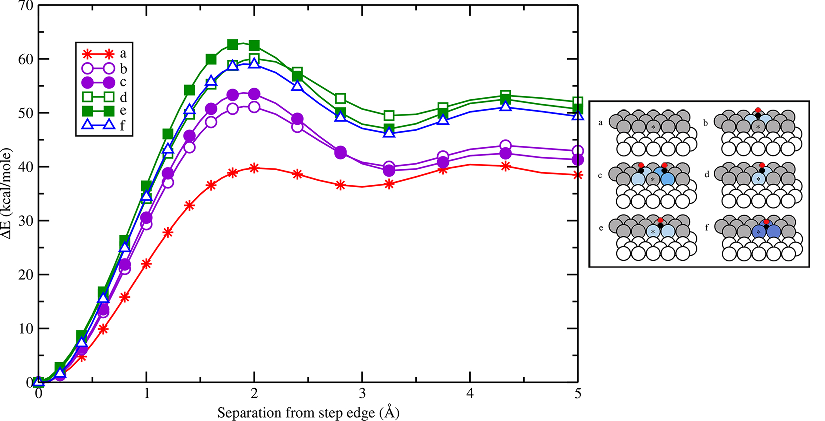
\includegraphics[width=0.9\linewidth]{../figures/chap3/PdEnergy_CO.pdf}
  \caption{The relative energies for moving a \ce{Pd} atom (marked
    with an asterisk) perpendicular to a (557) step edge. This atom is
    translated across the bare \ce{Pd} surface in curve A. The
    presence of one or two \ce{CO} molecules bound in bridge sites
    near the edge significantly stabilizes the edge atom (curves B and
    C).  If \ce{CO} is bound to the edge atom in either a bridge
    (curves D and E) or hollow (curve F) site, the barrier is
    increased.} \label{fig:PdEnergy}
\end{figure}
\end{landscape}

This \ce{CO}-induced step stabilization is significantly different
from the \ce{Pt\bond{-}CO} interaction which favors the atop binding
position. In the \ce{Pt\bond{-}CO} case, additional bound \ce{CO} on
the surface and has previously been shown to facilitate surface
roughening.\citep{Michalka:2013aa} The \ce{Pt\bond{-}CO} potential in
table~\ref{tab:CO_parameters} has been altered from the original
parameters in Ref. \citep{Michalka:2013aa}, and figure
\ref{fig:PtEnergy} shows that for the new potential, adsorbed \ce{CO}
can also disrupt step edges, providing an energetic benefit to
increasing the exposed \ce{Pt} surface area.

\begin{landscape}
\begin{figure}[p!]
  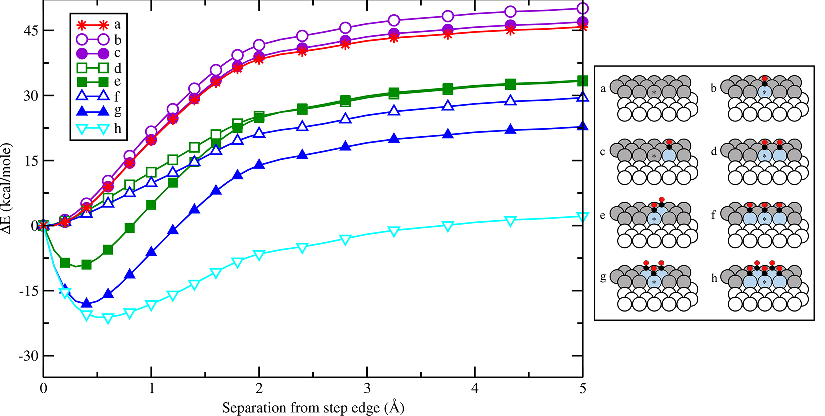
\includegraphics[width=0.9\linewidth]{../figures/chap3/PtEnergy_CO.pdf}
  \caption{The relative energies for moving a step-edge \ce{Pt} atom
    (marked with an asterisk) perpendicular to a (557) step edge.  As in
    figure \ref{fig:PdEnergy}, the bare surface is shown in curve A.
    The presence of atop-bound \ce{CO} molecules on the edge atom and
    at nearby sites can lower the energy for adatom formation
    (e.g. curves E, G, and H).} \label{fig:PtEnergy}
\end{figure}
\end{landscape}

Based on the curves in Figs. \ref{fig:PdEnergy} and
\ref{fig:PtEnergy}, the \ce{CO} adsorbates appear to increase the
surface energy of stepped \ce{Pd} surfaces and to lower the surface
energy of equivalent \ce{Pt} surfaces.  Therefore, a kinetic mechanism
seems to be the most reasonable explanation for the enhancement of island
formation.  By effectively lowering the surface energy of the \ce{Pt},
the bound \ce{CO} increases \ce{Pt}-atom mobility.  Once the mobile
\ce{Pt} atoms find nearby islands, the surface energies still favor
compact structures, and the islands can grow more rapidly. These
islands then sit on top of a \ce{CO}-stabilized \ce{Pd} substrate.
Additionally, since the modeled \ce{Pd\bond{-}CO} binding is somewhat
stronger than \ce{Pt\bond{-}CO}, island formation exposes more of the
\ce{Pd} substrate for energetically-favorable gas adsorption.

\section{Summary}

With the simulations we have performed on \ce{Pd} and \ce{Pt/Pd} (557)
surfaces, we have been able to model the formation of \ce{Pt} islands on the
surface of a catalytically interesting alloy. It was determined that the larger
surface energies of \ce{Pt} relative to \ce{Pd} favor the segregation of
\ce{Pt} into compact domains and the beginnings of island formation were
observed even without the \ce{CO} adsorbate present on the surface. This
restructuring was primarily kinetic in nature and the presence of \ce{CO}
increased the restructuring rate by roughening the step-edges and
destabilizing the surface which lowered the potential barriers. Conversely,
the bare \ce{Pd} surface was stabilized by the \ce{CO} adsorbate because of
the preferred bridge binding and thus maintained its (557) motif throughout
the simulations.

%Our primary conclusion is that the presence of chemisorbed carbon
%monoxide can speed up the formation of \ce{Pt} islands on the surface
%of a catalytically-interesting alloy, but that this effect is largely
%kinetic in nature.  The bare \ce{Pd} surface is stabilized by the
%\ce{CO} adsorbate, while stepped \ce{Pt} surfaces are roughened and
%destabilized by the presence of the same molecule. The larger surface
%energies of \ce{Pt} relative to \ce{Pd} already favor the segregation
%of \ce{Pt} into compact domains.  At elevated temperatures, we observe
%the beginnings of island formation even without the \ce{CO} adsorbate
%on the surface, which indicates that thermodynamics favors island
%formation on this surface.
%
%The energy profiles for step-edge adatom formation in the presence of
%adsorbed \ce{CO} (see figs. \ref{fig:PdEnergy} and \ref{fig:PtEnergy})
%would seem to bring the relative surface energies closer together in
%the presence of the adsorbed \ce{CO}. Thermodynamically, this should
%destabilize \ce{Pt} islands, so our observation that the 0.5 ML
%\ce{CO} speeds up the island-formation process appears to be due
%largely to kinetics.  The lower barriers for \ce{Pt}-adatom formation
%effectively speed up the surface diffusion of \ce{Pt}.  Previous work
%on \ce{Pt}(557) surfaces showed that \ce{CO} also lowers the barrier
%for a step-burrowing mechanism that can increase the thickness of
%\ce{Pt} surface layers.\citep{Michalka:2013aa}
%
%We note that there are other catalytically-active \ce{Pt}-alloys
%(notably \ce{PtNi3} and \ce{PtNi6} nanoparticles) that display
%dealloying of \ce{Pt} upon electrochemical cycling.\citep{Tuaev:2013fk}
%In analogy to the \ce{Pd} alloy studied here, the binding of \ce{CO}
%on \ce{Ni}(111) also prefers hollow sites in preference to atop
%locations.\citep{Campuzano:1979uq} However, the surface energies of
%\ce{Ni} are close to those of \ce{Pt}, so it is not clear if our
%conclusions about the \ce{Pd}/\ce{Pt} alloy would apply to this
%system.  Further research on these alloys would require adapting the
%\ce{M\bond{-}CO} models in order to predict whether carbon monoxide
%would be a generally effective tool for concentrating
%catalytically-active \ce{Pt} sites on surface alloys.


